\documentclass[]{tufte-book}

% ams
\usepackage{amssymb,amsmath}

\usepackage{ifxetex,ifluatex}
\usepackage{fixltx2e} % provides \textsubscript
\ifnum 0\ifxetex 1\fi\ifluatex 1\fi=0 % if pdftex
  \usepackage[T1]{fontenc}
  \usepackage[utf8]{inputenc}
\else % if luatex or xelatex
  \makeatletter
  \@ifpackageloaded{fontspec}{}{\usepackage{fontspec}}
  \makeatother
  \defaultfontfeatures{Ligatures=TeX,Scale=MatchLowercase}
  \makeatletter
  \@ifpackageloaded{soul}{
     \renewcommand\allcapsspacing[1]{{\addfontfeature{LetterSpace=15}#1}}
     \renewcommand\smallcapsspacing[1]{{\addfontfeature{LetterSpace=10}#1}}
   }{}
  \makeatother

\fi

% graphix
\usepackage{graphicx}
\setkeys{Gin}{width=\linewidth,totalheight=\textheight,keepaspectratio}

% booktabs
\usepackage{booktabs}

% url
\usepackage{url}

% hyperref
\usepackage{hyperref}

% units.
\usepackage{units}


\setcounter{secnumdepth}{-1}

% citations
\usepackage{natbib}
\bibliographystyle{plainnat}

% pandoc syntax highlighting

% longtable
\usepackage{longtable,booktabs}

% multiplecol
\usepackage{multicol}

% strikeout
\usepackage[normalem]{ulem}

% morefloats
\usepackage{morefloats}


% tightlist macro required by pandoc >= 1.14
\providecommand{\tightlist}{%
  \setlength{\itemsep}{0pt}\setlength{\parskip}{0pt}}

% title / author / date
\title{Estatística Descritiva}
\author{Rodrigo Citton P. dos Reis, Dep. de Estatística - UFRGS}
\date{Agosto de 2020}


\begin{document}

\maketitle




\hypertarget{introduuxe7uxe3o}{%
\chapter{Introdução}\label{introduuxe7uxe3o}}

\hypertarget{dados-leadsto-conhecimento}{%
\section{\texorpdfstring{Dados \(\leadsto\)
Conhecimento}{Dados \textbackslash leadsto Conhecimento}}\label{dados-leadsto-conhecimento}}

Em alguma fase de seu trabalho, o pesquisador depara-se com o problema
de \textbf{analisar} e \textbf{entender} um \textbf{conjunto de dados}
relevante ao seu particular objeto de estudos. Ele necessitará trabalhar
os dados para \textbf{transformá-los em informações}, para compará-los
com outros resultados, ou ainda para \textbf{julgar sua adequação} a
\textbf{alguma teoria}.

Uma representação

\begin{center}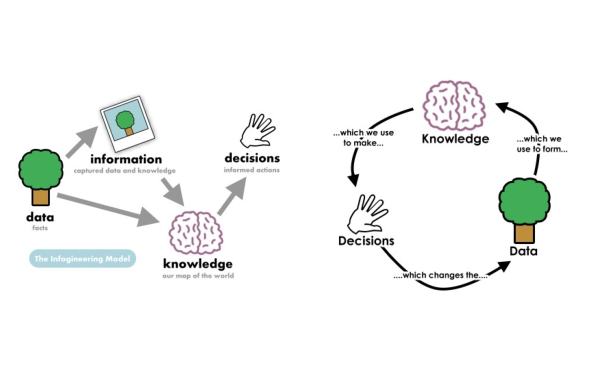
\includegraphics[width=1\linewidth,height=0.8\textheight]{conceitos_basicos_files/figure-latex/unnamed-chunk-1-1} \end{center}

Uma representação mais ousada!

\begin{center}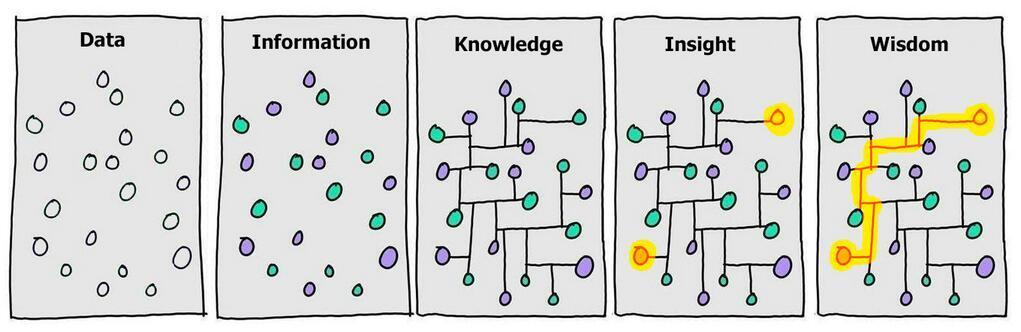
\includegraphics[width=1\linewidth]{C:/Users/rodri/OneDrive/Documentos/UFRGS/Disciplinas/estatistica_descritiva/MAT02018/images/Data-Wisdom} \end{center}

\hypertarget{o-muxe9todo-cientuxedfico}{%
\section{O Método Científico}\label{o-muxe9todo-cientuxedfico}}

De modo bem geral, podemos dizer que a essência da Ciência é a
\textbf{observação} e que seu objetivo básico é a \textbf{inferência}.

\begin{center}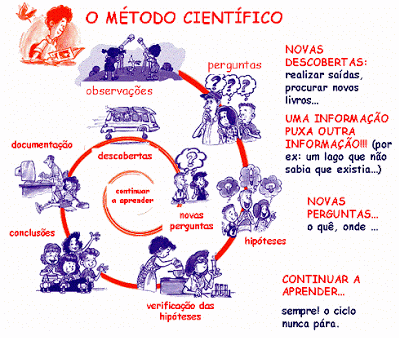
\includegraphics[width=0.7\linewidth,height=0.7\textheight]{C:/Users/rodri/OneDrive/Documentos/UFRGS/Disciplinas/estatistica_descritiva/MAT02018/images/metodo} \end{center}

De modo bem geral, podemos dizer que a essência do Aprendizado (da
Evolução).

\begin{center}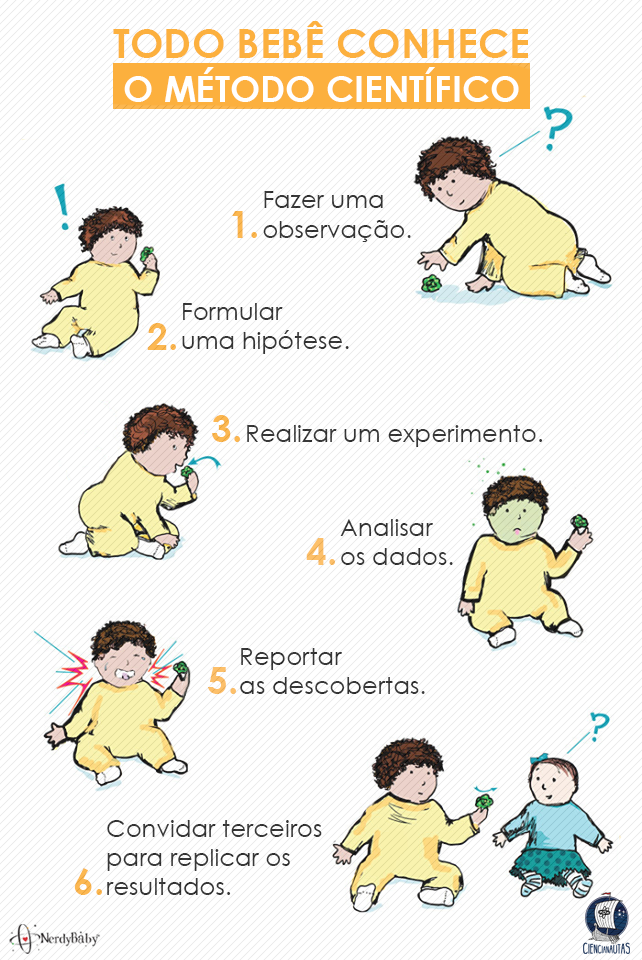
\includegraphics[width=0.5\linewidth,height=0.7\textheight]{C:/Users/rodri/OneDrive/Documentos/UFRGS/Disciplinas/estatistica_descritiva/MAT02018/images/metodo_cientifico_bebes} \end{center}

\hypertarget{conceitos-buxe1sicos}{%
\chapter{Conceitos básicos}\label{conceitos-buxe1sicos}}

\hypertarget{o-que-uxe9-a-estatuxedstica}{%
\section{O que é a estatística?}\label{o-que-uxe9-a-estatuxedstica}}

A \textbf{estatística}\footnote{Do grego \emph{statistós}, de
  \emph{statízo}, \textbf{``estabelecer''}, \textbf{``verificar''},
  acrescido do sufixo \emph{ica}.} é a ciência que tem por objetivo
orientar a coleta, o resumo, a apresentação, a análise e a interpretação
de dados. Podem ser identificadas duas grandes áreas de atuação desta
ciência:

\begin{itemize}
\tightlist
\item
  a \textbf{estatística descritiva}, envolvida com o resumo e a
  apresentação dos dados.
\item
  a \textbf{estatística inferencial}, que ajuda a concluir sobre
  conjuntos maiores de dados (populações) quando apenas partes desses
  conjuntos (as amostras) foram estudadas. 
\end{itemize}

\begin{center}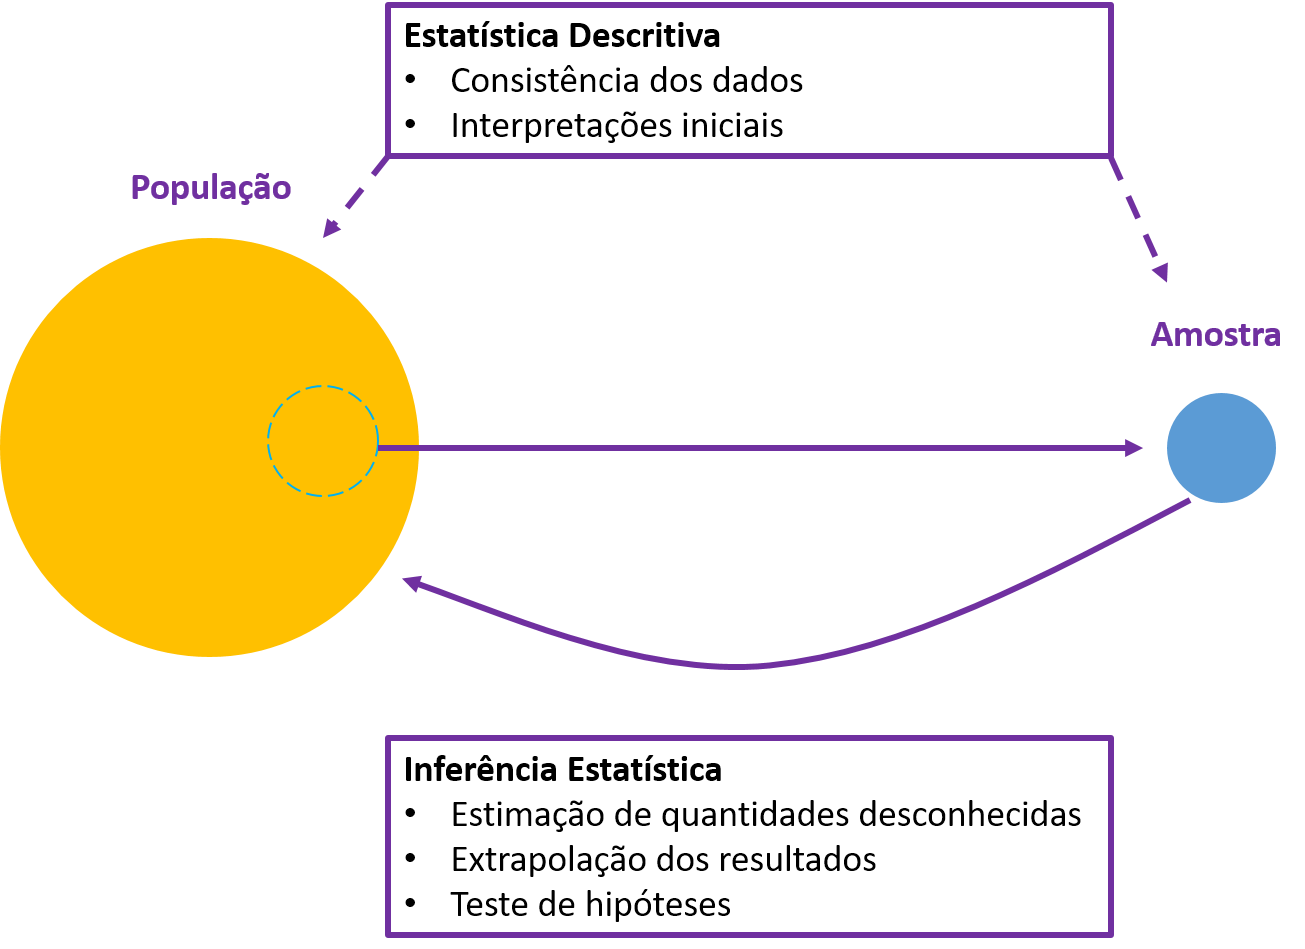
\includegraphics[width=1\linewidth,height=0.8\textheight]{C:/Users/rodri/OneDrive/Documentos/UFRGS/Disciplinas/estatistica_descritiva/MAT02018/images/Descritiva_Inferencia} \end{center}

\hypertarget{o-que-uxe9-a-estatuxedstica-descritiva}{%
\section{O que é a estatística
descritiva?}\label{o-que-uxe9-a-estatuxedstica-descritiva}}

A \textbf{Estatística Descritiva} corresponde aos procedimentos
relacionados com a \textbf{coleta}, \textbf{elaboração},
\textbf{tabulação}, \textbf{análise}, \textbf{interpretação} e
\textbf{apresentação} dos \textbf{dados}. Isto é, inclui as técnicas que
dizem respeito à sintetização e à descrição de dados numéricos. Estas
técnicas podem ser utilizadas em pelo menos dois contextos:

\begin{itemize}
\tightlist
\item
  Análise da \textbf{consistência dos dados}.
\item
  \textbf{Análise Exploratória de Dados} (\emph{Exploratory Data
  Analysis} - EDA)\footnote{Tukey, J. W. \emph{Exploratory data
    analysis}, Reading:Addison-Wesley, 1977.}.
\end{itemize}

Tais métodos tanto podem ser gráficos como envolver análise
computacional.

\hypertarget{estatuxedstica-descritiva-alguns-exemplos}{%
\section{Estatística descritiva: alguns
exemplos}\label{estatuxedstica-descritiva-alguns-exemplos}}

\hypertarget{descriptive-statistics}{%
\subsection{Descriptive Statistics}\label{descriptive-statistics}}

\hypertarget{tobacco}{%
\subsubsection{tobacco}\label{tobacco}}

\textbf{N:} 1000

\begin{longtable}[]{@{}rrrrr@{}}
\toprule
~ & age & BMI & cigs.per.day & samp.wgts\tabularnewline
\midrule
\endhead
\textbf{Mean} & 49.60 & 25.73 & 6.78 & 1.00\tabularnewline
\textbf{Std.Dev} & 18.29 & 4.49 & 11.88 & 0.08\tabularnewline
\textbf{Min} & 18.00 & 8.83 & 0.00 & 0.86\tabularnewline
\textbf{Q1} & 34.00 & 22.93 & 0.00 & 0.86\tabularnewline
\textbf{Median} & 50.00 & 25.62 & 0.00 & 1.04\tabularnewline
\textbf{Q3} & 66.00 & 28.65 & 11.00 & 1.05\tabularnewline
\textbf{Max} & 80.00 & 39.44 & 40.00 & 1.06\tabularnewline
\textbf{MAD} & 23.72 & 4.18 & 0.00 & 0.01\tabularnewline
\textbf{IQR} & 32.00 & 5.72 & 11.00 & 0.19\tabularnewline
\textbf{CV} & 0.37 & 0.17 & 1.75 & 0.08\tabularnewline
\textbf{Skewness} & -0.04 & 0.02 & 1.54 & -1.04\tabularnewline
\textbf{SE.Skewness} & 0.08 & 0.08 & 0.08 & 0.08\tabularnewline
\textbf{Kurtosis} & -1.26 & 0.26 & 0.90 & -0.90\tabularnewline
\textbf{N.Valid} & 975.00 & 974.00 & 965.00 & 1000.00\tabularnewline
\textbf{Pct.Valid} & 97.50 & 97.40 & 96.50 & 100.00\tabularnewline
\bottomrule
\end{longtable}

\begin{longtable}[]{@{}rrrrrr@{}}
\toprule
~ & Freq & \% Valid & \% Valid Cum. & \% Total & \% Total
Cum.\tabularnewline
\midrule
\endhead
\textbf{F} & 489 & 50.00 & 50.00 & 48.90 & 48.90\tabularnewline
\textbf{M} & 489 & 50.00 & 100.00 & 48.90 & 97.80\tabularnewline
\textbf{\textless NA\textgreater{}} & 22 & & & 2.20 &
100.00\tabularnewline
\textbf{Total} & 1000 & 100.00 & 100.00 & 100.00 & 100.00\tabularnewline
\bottomrule
\end{longtable}

\begin{center}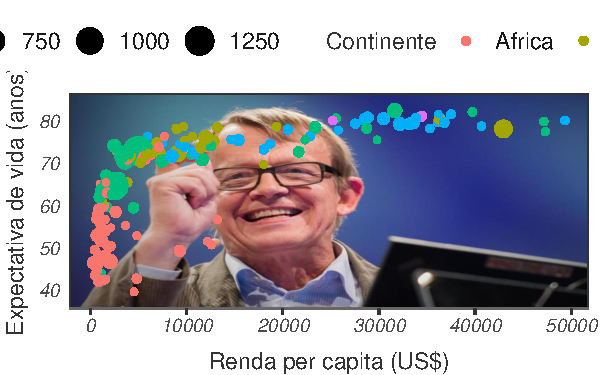
\includegraphics[width=0.95\linewidth]{conceitos_basicos_files/figure-latex/unnamed-chunk-8-1} \end{center}

\hypertarget{unidades-experimentais-e-observacionais}{%
\section{Unidades experimentais e
observacionais}\label{unidades-experimentais-e-observacionais}}

\textbf{Unidade experimental} ou \textbf{unidade de observação} é a
menor unidade a fornecer informação.

\begin{itemize}
\tightlist
\item
  \textbf{Ex:} alunos, pacientes, animais, plantas, carros, hospitais,
  escolas, cidades, universidades, países, \emph{tweets}, etc.
\end{itemize}

\hypertarget{crash-course-de-inferuxeancia-causal}{%
\subsection{Crash course de inferência
causal}\label{crash-course-de-inferuxeancia-causal}}

\begin{itemize}
\tightlist
\item
  \textbf{Qual o melhor tratamento para o choque séptico?}
\end{itemize}

Dois tipos de estudo podem ser conduzidos para responder a esta questão
de pesquisa:

\begin{enumerate}
\def\labelenumi{\arabic{enumi}.}
\tightlist
\item
  Em um \textbf{experimento aleatorizado} (\emph{randomized trial}), uma
  moeda justa é lançada repetidamente para designar o tratamento de cada
  paciente.
\item
  Um \textbf{estudo observacional} é uma investigação empírica em que o
  objetivo é elucidar relações de causa e efeito, em que não é factível
  o uso de experimentação controlada, no sentido de ser capaz de impor
  procedimentos ou tratamentos cujos os efeitos se deseja descobrir.
\end{enumerate}

\hypertarget{experimentos-exemplo}{%
\subsection{Experimentos: exemplo}\label{experimentos-exemplo}}

\begin{itemize}
\tightlist
\item
  ``O chá servido sobre o leite parecia ficar com gosto diferente do que
  apresentava ao receber o leite sobre ele''\footnote{Salsburg, D.
    \emph{Uma senhora toma chá \ldots{} como a estatística revolucionou
    a ciência no século XX}, Zahar, 2009.}.
\end{itemize}

\begin{center}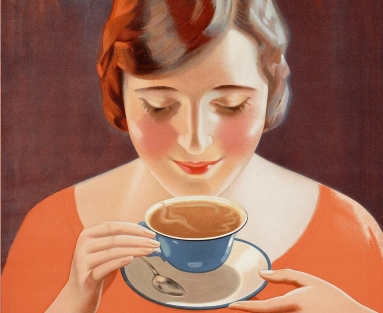
\includegraphics[width=0.7\linewidth,height=0.6\textheight]{C:/Users/rodri/OneDrive/Documentos/UFRGS/Disciplinas/estatistica_descritiva/MAT02018/images/uma_senhora_toma_cha} \end{center}

\hypertarget{estudos-observacionais-exemplo}{%
\subsection{Estudos observacionais:
exemplo}\label{estudos-observacionais-exemplo}}

\begin{itemize}
\tightlist
\item
  ``O \textbf{Ministério da Saúde} adverte: \textbf{fumar pode causar
  câncer de pulmão}''.
\end{itemize}

\begin{center}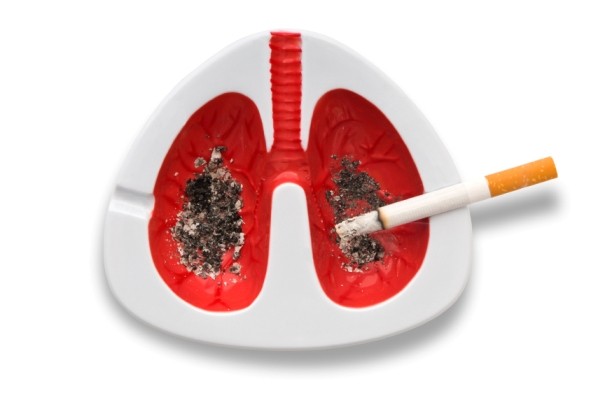
\includegraphics[width=0.7\linewidth]{C:/Users/rodri/OneDrive/Documentos/UFRGS/Disciplinas/estatistica_descritiva/MAT02018/images/smokingAndLungCancer2} \end{center}

\begin{verbatim}
1. Elabore uma questão de pesquisa de seu interesse (anote a sua questão em algum lugar).
2. Discuta a respeito da sua questão de pesquisa com os colegas.
\end{verbatim}

\hypertarget{dados-e-variuxe1veis}{%
\section{Dados e variáveis}\label{dados-e-variuxe1veis}}

\begin{block}

\hypertarget{dados}{%
\subsection{Dados}\label{dados}}

São as informações obtidas de uma unidade experimental ou
observacional.\\

\begin{itemize}
\tightlist
\item
  \textbf{Ex:} ``Vitor tem 25 anos e é fumante''. Os dados são ``25
  anos'' e ``fumante''.
\end{itemize}

\end{block}

\begin{block}

\hypertarget{variuxe1vel}{%
\subsection{Variável}\label{variuxe1vel}}

É toda característica que, observada em uma unidade (experimental ou
observacional), pode variar de um indivíduo para outro.\\

\begin{itemize}
\tightlist
\item
  \textbf{Ex:} idade, sexo, altura, nível de hemoglobina no sangue,
  espaçamento entre plantas, doses de um medicamento, tipo de
  medicamento, cultivares, número de caracteres, velocidade da rede,
  tempo gasto na rede social, nível de monóxido de carbono em emissões
  do escape de automóveis, etc.
\end{itemize}

\end{block}

É importante \textbf{identificar que tipo de variável} está sendo
estudada, uma vez que são recomendados \textbf{procedimentos
estatísticos diferentes} em cada situação.

\hypertarget{tipos-de-variuxe1veis}{%
\section{Tipos de variáveis}\label{tipos-de-variuxe1veis}}

\begin{center}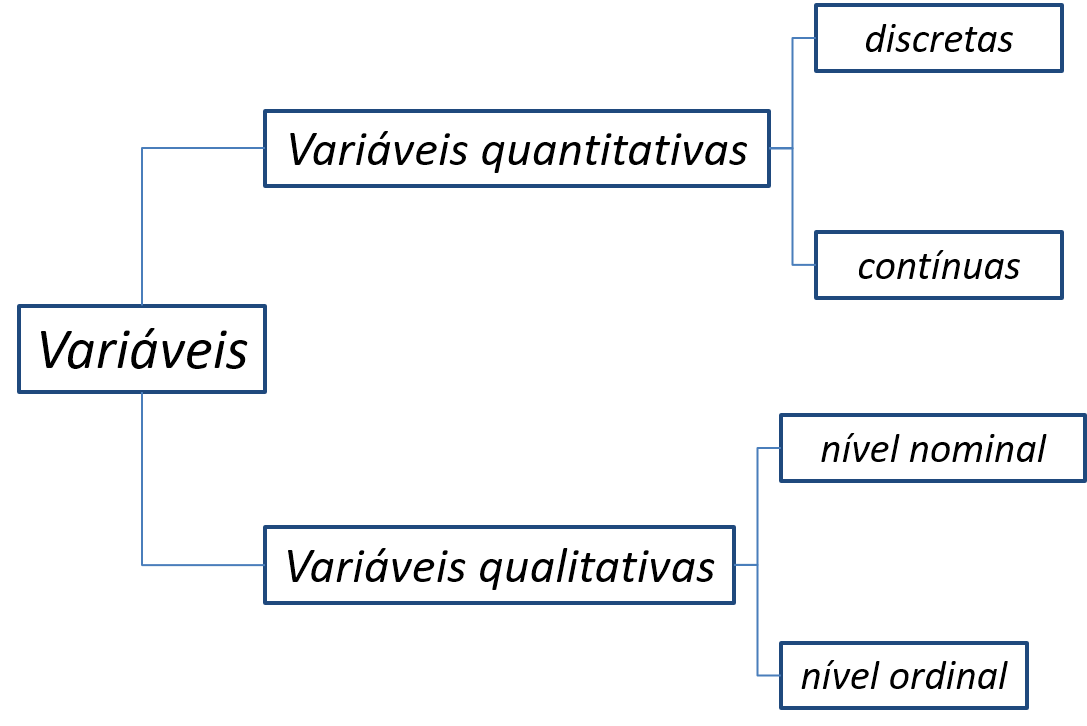
\includegraphics[width=0.9\linewidth]{C:/Users/rodri/OneDrive/Documentos/UFRGS/Disciplinas/estatistica_descritiva/MAT02018/images/classe_var} \end{center}

\hypertarget{variuxe1veis-quantitativas}{%
\section{Variáveis quantitativas}\label{variuxe1veis-quantitativas}}

\begin{center}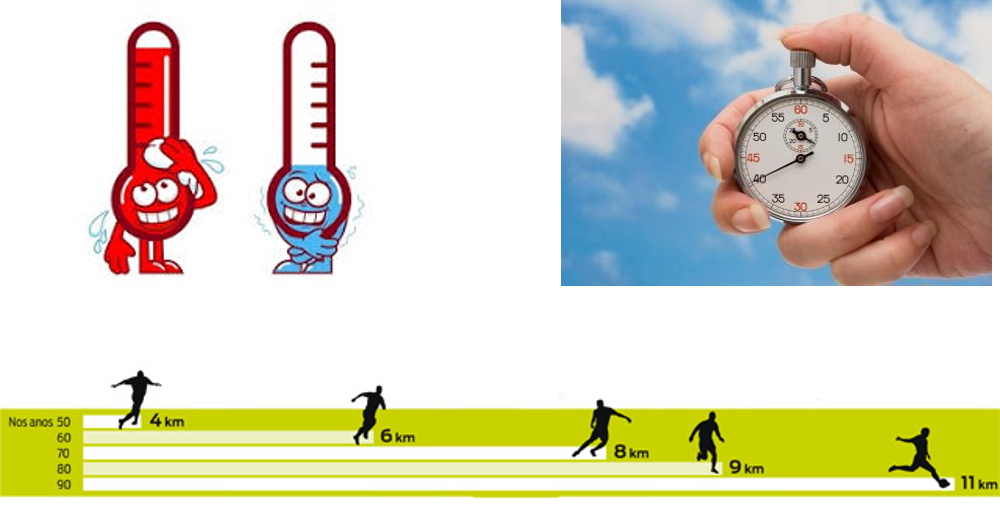
\includegraphics[width=1\linewidth]{C:/Users/rodri/OneDrive/Documentos/UFRGS/Disciplinas/estatistica_descritiva/MAT02018/images/var_quanti} \end{center}

\hypertarget{variuxe1veis-quantitativas-discretas}{%
\section{Variáveis quantitativas
discretas}\label{variuxe1veis-quantitativas-discretas}}

\begin{center}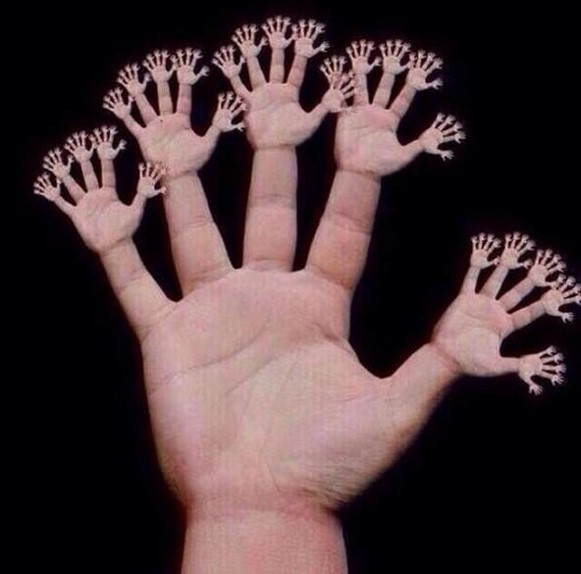
\includegraphics[width=0.6\linewidth]{C:/Users/rodri/OneDrive/Documentos/UFRGS/Disciplinas/estatistica_descritiva/MAT02018/images/var_discreta} \end{center}

\hypertarget{variuxe1veis-quantitativas-contuxednuas}{%
\section{Variáveis quantitativas
contínuas}\label{variuxe1veis-quantitativas-contuxednuas}}

\begin{center}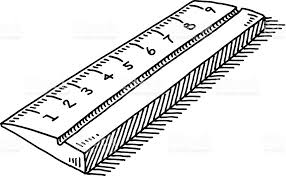
\includegraphics[width=0.7\linewidth]{C:/Users/rodri/OneDrive/Documentos/UFRGS/Disciplinas/estatistica_descritiva/MAT02018/images/var_continua} \end{center}

\hypertarget{variuxe1veis-qualitativas}{%
\section{Variáveis qualitativas}\label{variuxe1veis-qualitativas}}

\begin{center}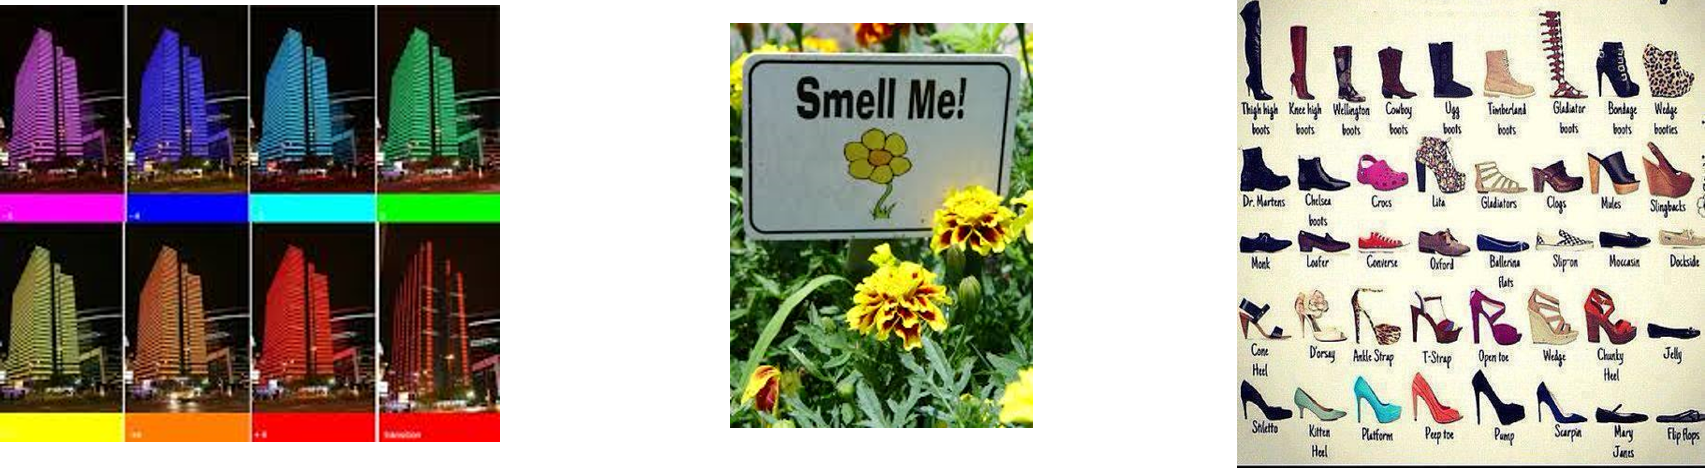
\includegraphics[width=1\linewidth]{C:/Users/rodri/OneDrive/Documentos/UFRGS/Disciplinas/estatistica_descritiva/MAT02018/images/var_quali} \end{center}

\hypertarget{variuxe1veis-qualitativas-ordinais}{%
\section{Variáveis qualitativas
ordinais}\label{variuxe1veis-qualitativas-ordinais}}

\begin{center}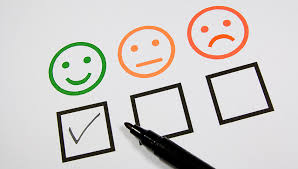
\includegraphics[width=1\linewidth]{C:/Users/rodri/OneDrive/Documentos/UFRGS/Disciplinas/estatistica_descritiva/MAT02018/images/var_ordinal} \end{center}

\hypertarget{variuxe1veis-qualitativas-nominais}{%
\section{Variáveis qualitativas
nominais}\label{variuxe1veis-qualitativas-nominais}}

\begin{center}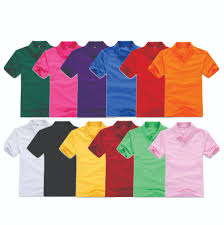
\includegraphics[width=0.7\linewidth]{C:/Users/rodri/OneDrive/Documentos/UFRGS/Disciplinas/estatistica_descritiva/MAT02018/images/var_nominal} \end{center}

\hypertarget{exemplos-1}{%
\section{Exemplos (1)}\label{exemplos-1}}

\begin{center}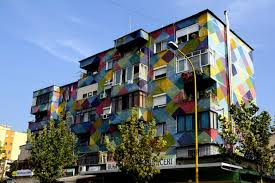
\includegraphics[width=0.9\linewidth]{C:/Users/rodri/OneDrive/Documentos/UFRGS/Disciplinas/estatistica_descritiva/MAT02018/images/cor_predio2} \end{center}

\hypertarget{exemplos-1-1}{%
\section{Exemplos (1)}\label{exemplos-1-1}}

\hypertarget{variuxe1veis-quantitativas-1}{%
\subsection{Variáveis
quantitativas}\label{variuxe1veis-quantitativas-1}}

\begin{itemize}
\tightlist
\item
  3 andares
\item
  14,85 metros de altura
\end{itemize}

\hypertarget{variuxe1veis-qualitativas-1}{%
\subsection{Variáveis qualitativas}\label{variuxe1veis-qualitativas-1}}

\begin{itemize}
\tightlist
\item
  Multicolorido
\item
  Cheira ``bem''
\end{itemize}

\hypertarget{exemplos-2}{%
\section{Exemplos (2)}\label{exemplos-2}}

\begin{center}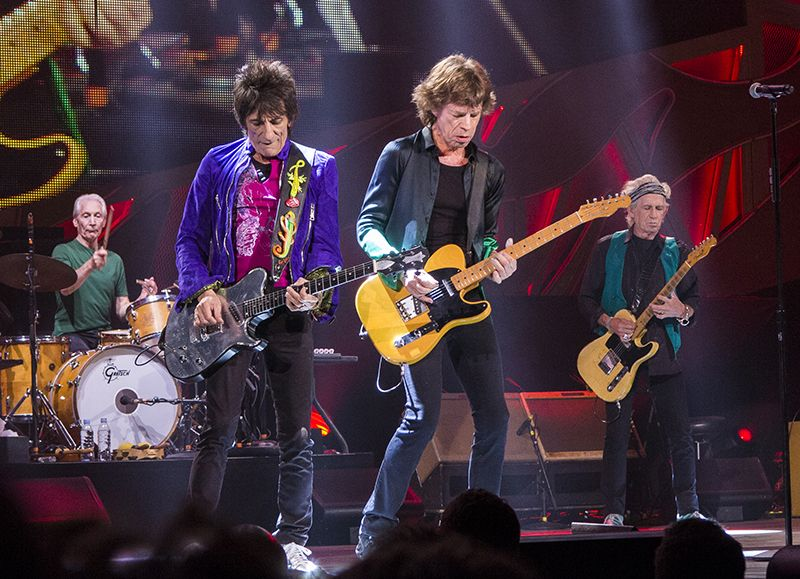
\includegraphics[width=0.9\linewidth]{C:/Users/rodri/OneDrive/Documentos/UFRGS/Disciplinas/estatistica_descritiva/MAT02018/images/rolling-stones} \end{center}

\hypertarget{exemplos-2-1}{%
\section{Exemplos (2)}\label{exemplos-2-1}}

\hypertarget{variuxe1veis-quantitativas-2}{%
\subsection{Variáveis
quantitativas}\label{variuxe1veis-quantitativas-2}}

\begin{itemize}
\tightlist
\item
  4 integrantes
\item
  56 anos
\end{itemize}

\hypertarget{variuxe1veis-qualitativas-2}{%
\subsection{Variáveis qualitativas}\label{variuxe1veis-qualitativas-2}}

\begin{itemize}
\tightlist
\item
  Inglaterra
\item
  Rock
\end{itemize}

\hypertarget{exercuxedcio}{%
\section{Exercício}\label{exercuxedcio}}

\begin{enumerate}
\def\labelenumi{\arabic{enumi}.}
\tightlist
\item
  Com base na questão de pesquisa elaborada no exercício anterior, liste
  variáveis que você teria interesse em coletar e analisar para
  responder a sua questão de pesquisa.
\item
  Classifique as variáveis de acordo com a classificação discutida
  anteriormente.
\item
  Discuta a respeito das suas variáveis com os colegas.
\end{enumerate}

\hypertarget{populauxe7uxe3o}{%
\section{População}\label{populauxe7uxe3o}}

\begin{itemize}
\tightlist
\item
  \textbf{População} ou \textbf{universo}: esse termo é usado em
  estatística com um sentido bem mais amplo do que na linguagem
  coloquial.
\item
  É entendido aqui como o \textbf{conjunto de todos os elementos} que
  apresentam uma ou mais características \textbf{em comum}.
\item
  \textbf{Exemplo 1:} a população de colegiais de oito anos de Belo
  Horizonte.

  \begin{itemize}
  \tightlist
  \item
    Estes colegiais têm em comum a idade e o local onde vivem.
  \end{itemize}
\item
  \textbf{Exemplo 2:} a população de indústrias brasileiras.

  \begin{itemize}
  \tightlist
  \item
    Estas indústrias têm em comum o fato de que foram criadas no Brasil.
  \end{itemize}
\item
  Este conjunto por vezes é denominado por \(U\) (de \textbf{conjunto
  universo}).
\item
  O \textbf{tamanho da população} é a sua quantidade de elementos, que
  anotamos por \(N\).
\item
  Uma população pode ser \textbf{finita} (limita em tamanho;
  \(N < \infty\)) ou \textbf{infinita} (\(N =\infty\)).

  \begin{itemize}
  \tightlist
  \item
    \textbf{Exemplo de pop. finita:} torcedores do São Raimundo de
    Santarém, residentes de Porto Alegre.
  \item
    \textbf{Exemplo de pop. infinita:} equipamentos (de um certo tipo)
    fabricados em série.
  \end{itemize}
\end{itemize}

\hypertarget{censo-e-amostra}{%
\section{Censo e amostra}\label{censo-e-amostra}}

\begin{itemize}
\tightlist
\item
  Quando o estudo é realizado com toda a população de interesse,
  chamemos este estudo de \textbf{censo}.
\item
  Por motivos de tempo, custo, logística, entre outros, geralmente não é
  possível realizar um censo.

  \begin{itemize}
  \tightlist
  \item
    Nestes casos, estudamos apenas uma parcela da população, que
    chamamos de \textbf{amostra}.
  \end{itemize}
\end{itemize}

\hypertarget{censo-vs.-amostra}{%
\subsection{Censo vs.~amostra}\label{censo-vs.-amostra}}

À primeira vista, uma coleta de dados realizada em toda a população é
preferível a uma realizada apenas numa parte da população. Na prática,
entretanto, o oposto é frequentemente verdadeiro porque:

\begin{enumerate}
\def\labelenumi{\arabic{enumi}.}
\tightlist
\item
  Um censo é impossível quando a população é infinita.
\item
  Os ensaios (testes) podem ser destrutivos
  \structure{(como nos testes de segurança dos carros)}.
\item
  Rapidez: estudar toda a população pode despender de muito tempo, não
  sendo compatível com a urgência do estudo
  \structure{(como quando estudamos os casos de um surto de uma nova doença)}.
\end{enumerate}

Para uma consideração mais completa ver Vargas
(2000)\footnote{Vargas, J. B. \emph{Estatística: uma linguagem para dialogar com a incerteza}, Cadernos de matemática e estatística. Série B, 2000.}.

\hypertarget{amostra}{%
\section{Amostra}\label{amostra}}

\begin{itemize}
\tightlist
\item
  \textbf{Amostra} é qualquer fração de uma população.

  \begin{itemize}
  \tightlist
  \item
    Como sua finalidade é representar a população, deseja-se que a
    amostra escolhida apresente as mesmas características da população
    de origem, isto é, que seja uma amostra \textbf{``representativa''}
    ou \textbf{``não-tendenciosa''}.
  \end{itemize}
\item
  Tanto o número de indivíduos selecionados para a amostra quanto a
  técnica de seleção são extremamente importantes para que os resultados
  obtidos no estudo sejam generalizados para a população.
\end{itemize}

\hypertarget{amostra-representativa}{%
\section{Amostra representativa}\label{amostra-representativa}}

\begin{center}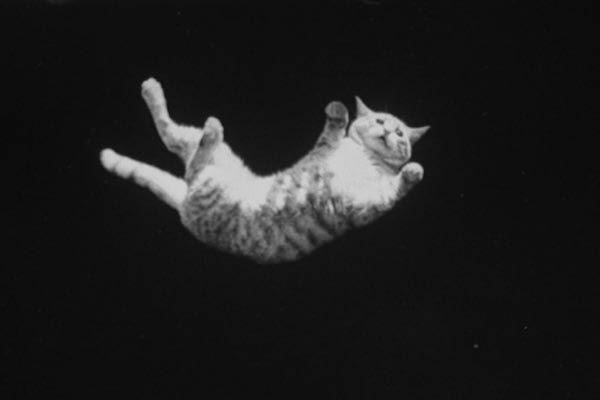
\includegraphics[width=0.65\linewidth]{C:/Users/rodri/OneDrive/Documentos/UFRGS/Disciplinas/estatistica_descritiva/MAT02018/images/Gato_caindo} \end{center}

\begin{itemize}
\tightlist
\item
  Ver a discussão sobre \textbf{representatividade da amostra} na
  \href{https://www.youtube.com/watch?v=TGGGDpb04Yc\&t=592s}{apresentação}
  do \textbf{Prof.~Chris Fonnesbeck}.
\end{itemize}

\hypertarget{amostragem}{%
\section{Amostragem}\label{amostragem}}

\begin{itemize}
\tightlist
\item
  A seleção da amostra pode ser feita de várias maneiras.
\item
  Esta dependerá:

  \begin{itemize}
  \tightlist
  \item
    Do grau de conhecimento que temos da população.
  \item
    Da quantidade de recursos disponíveis.
  \end{itemize}
\item
  A seleção da amostra tenta fornecer um subconjunto de valores o
  \textbf{mais parecido possível} com a população que lhe dá origem.

  \begin{itemize}
  \tightlist
  \item
    \textbf{Amostra representativa} da população.
  \end{itemize}
\end{itemize}

\hypertarget{amostra-aleatuxf3ria-simples}{%
\section{Amostra aleatória simples}\label{amostra-aleatuxf3ria-simples}}

\begin{itemize}
\tightlist
\item
  A amostragem mais usada é a \textbf{amostra casual simples} (ou
  aleatória simples).

  \begin{itemize}
  \tightlist
  \item
    Os indivíduos (unidades) da amostra são selecionados ao acaso,
    \textbf{com} ou \textbf{sem reposição}.
  \end{itemize}
\end{itemize}

\begin{center}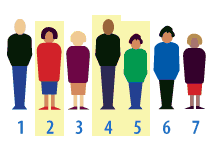
\includegraphics[width=0.6\linewidth]{C:/Users/rodri/OneDrive/Documentos/UFRGS/Disciplinas/estatistica_descritiva/MAT02018/images/simpleSample} \end{center}

\hypertarget{amostra-estratificada}{%
\section{Amostra estratificada}\label{amostra-estratificada}}

\begin{itemize}
\item
  Eventualmente, se tivermos informações adicionais a respeito da
  população de interesse, podemos utilizar outros esquemas de amostragem
  mais sofisticados.

  \begin{itemize}
  \tightlist
  \item
    \textbf{Amostragem estratificada}
  \end{itemize}
\end{itemize}

\begin{center}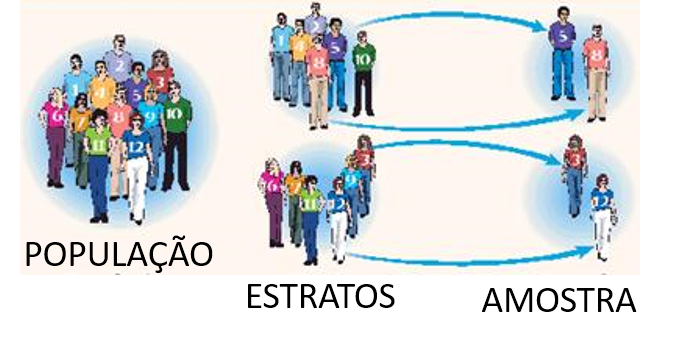
\includegraphics[width=0.95\linewidth]{C:/Users/rodri/OneDrive/Documentos/UFRGS/Disciplinas/estatistica_descritiva/MAT02018/images/estratificada} \end{center}

\hypertarget{amostra-sistemuxe1tica}{%
\section{Amostra sistemática}\label{amostra-sistemuxe1tica}}

\begin{itemize}
\tightlist
\item
  Em outros casos, pode existir uma relação numerada dos itens da
  população que nos permitiria utilizar a chamada \textbf{amostragem
  sistemática} em que selecionamos os indivíduos de forma
  pré-determinada.
\end{itemize}

\begin{center}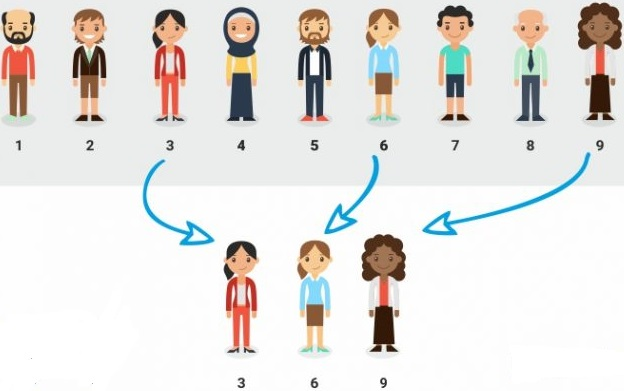
\includegraphics[width=0.8\linewidth]{C:/Users/rodri/OneDrive/Documentos/UFRGS/Disciplinas/estatistica_descritiva/MAT02018/images/SystematicSampling} \end{center}

\hypertarget{amostragem-1}{%
\section{Amostragem}\label{amostragem-1}}

\begin{itemize}
\tightlist
\item
  Outros esquemas de amostragem poderiam ser citados e todos fazem parte
  da chamada \textbf{teoria da amostragem}, cujos detalhes não serão
  aprofundados.
\end{itemize}

\hypertarget{paruxe2metros-estatuxedsticas-e-estimativas}{%
\section{Parâmetros, estatísticas e
estimativas}\label{paruxe2metros-estatuxedsticas-e-estimativas}}

\begin{itemize}
\tightlist
\item
  \textbf{Parâmetro} é um valor que resume, na população, a informação
  relativa a uma variável.

  \begin{itemize}
  \tightlist
  \item
    \textbf{Ex:} média populacional, prevalência populacional,
    coeficiente de variação populacional, taxa de mortalidade
    populacional, etc.
  \end{itemize}
\item
  \textbf{Estatística} (além de ser o nome da ciência/área do
  conhecimento) é a denominação dada a uma quantidade, calculada com
  base nos elementos de uma amostra, que descreve a informação contida
  nesse conjunto de dados.

  \begin{itemize}
  \tightlist
  \item
    \textbf{Ex:} A média, a porcentagem, o desvio padrão, o coeficiente
    de correlação, calculados em uma amostra, são estatísticas.
  \end{itemize}
\end{itemize}

\hypertarget{paruxe2metros-estatuxedsticas-e-estimativas-1}{%
\section{Parâmetros, estatísticas e
estimativas}\label{paruxe2metros-estatuxedsticas-e-estimativas-1}}

\begin{itemize}
\tightlist
\item
  Os parâmetros são difíceis de se obter, pois implicam o estudo de toda
  a população e costumam ser substituídos por valores calculados em
  amostras representativas da população-alvo.

  \begin{itemize}
  \tightlist
  \item
    Se tivesse sido examinada uma amostra de 10 estudantes matriculados
    na disciplina MAT02218, e 40\% fossem do torcedores do América
    Mineiro, esse valor constituiria uma estimativa do parâmetro
    ``percentual de torcedores do América Mineiro matriculados naquela
    disciplina''.
  \end{itemize}
\item
  A \textbf{estimativa} é um valor numérico de uma estatística, usado
  para realizar inferências sobre o parâmetro.

  \begin{itemize}
  \tightlist
  \item
    Da mesma forma, o valor numérico da média para a estatura desses 10
    alunos, digamos 173 cm, é uma estimativa para a média de altura
    populacional.
  \end{itemize}
\item
  \textbf{P:} neste exemplo, quem é a população (alvo)?
\end{itemize}

\hypertarget{pruxf3xima-aula}{%
\section{Próxima aula}\label{pruxf3xima-aula}}

\begin{itemize}
\tightlist
\item
  Organização dos dados 
\end{itemize}

\hypertarget{para-casa}{%
\section{Para casa}\label{para-casa}}

\begin{columns}[c]
\column{2.3in}
\begin{figure}[!h]
\begin{center}
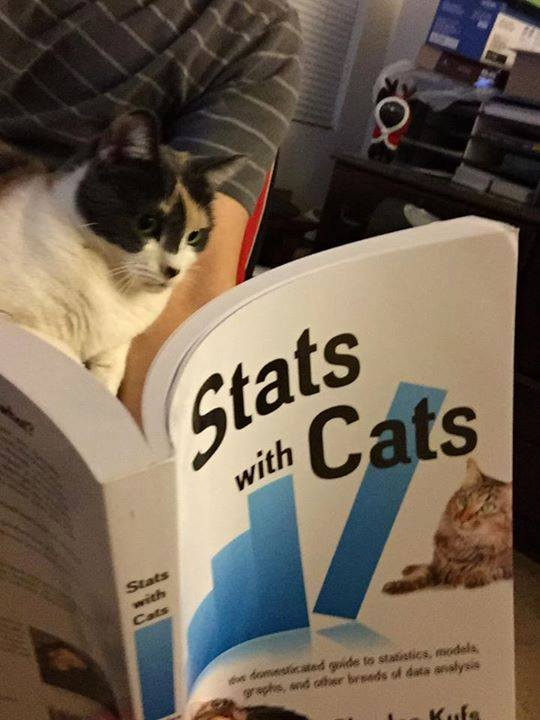
\includegraphics[width=0.9\columnwidth]{images/stats_cats.jpg}
\end{center}
\end{figure}
\column{2.3in}
\begin{itemize}\setlength{\itemsep}{+2mm}
\item Conhecer o Moodle da disciplina.
\item Ler os Cap. 1 e 2 de "Estatística Descritiva I" de Fernandez.
\end{itemize}
\end{columns}

\hypertarget{por-hoje-uxe9-suxf3-bons-estudos}{%
\section{Por hoje é só! Bons
estudos!}\label{por-hoje-uxe9-suxf3-bons-estudos}}

\begin{center}
\includegraphics[width=1\linewidth,height=0.8\textheight]{C:/Users/rodri/OneDrive/Documentos/UFRGS/Disciplinas/estatistica_descritiva/MAT02018/images/lofi_01} \end{center}

\bibliography{skeleton.bib}



\end{document}
